\section*{Comparación de algoritmos}

En esta sección, nos concentramos en la implementación de diferentes algoritmos de clasificación, para luego testear la performance de cada uno de ellos.
En particular, utilizamos los algoritmos de \textit{K-vecinos Más Cercanos} (KNN), \textit{Support Vector Machine} (SVM) y \textit{Árboles de Decisión}. 
A su vez, en cada uno de estos algoritmos, realizamos una búsqueda de hiperparámetros, utilizando Randomized Search, para encontrar la mejor combinación
posible.

\subsection*{Árboles de decisión}
Para árboles de decisión, decidimos utilizar los siguientes hiperparámetros para realizar la búsqueda:
\begin{itemize}
    \item \texttt{max\_depth}: Profundidad máxima del árbol. Probamos un rango de alturas entre 1 y 25, teniendo en cuenta que la altura del árbol balanceado sería $log_2(425) = 9$.
    \item\texttt{Criterion}: los vistos en clase, \textit{Gini} y \textit{Entropy}, y \textit{log loss}.

    \item \texttt{min\_samples\_split}: Número mínimo de muestras requeridas para dividir un nodo.
    
    \item \texttt{min\_samples\_leaf}: Número mínimo de muestras requeridas para estar en una hoja.
    
    \item \texttt{max\_features}: Número máximo de características a considerar al buscar la mejor división. En este caso, probamos con un máximo de 1, 3, sqrt y log$_2$, e ilimitado.
\end{itemize}

Las 6 mejores configuraciones obtenidas respecto a la métrica \textit{AUC-ROC} fueron las siguientes:

\begin{table}[H]
    \centering
    \begin{tabular}{|l|c|c|c|c|c|c|}
    \hline
    \textbf{Modelo} & \textbf{Min Samples Split} & \textbf{Min Samples Leaf} & \textbf{Max Features} & \textbf{Max Depth} & \textbf{Criterion} & \textbf{AUC-ROC} \\
    \hline
    \rowcolor{yellow!30}
    Árbol 1 & 10 & 4 & none & 6 & entropy & 0.646 \\
    Árbol 2 & 5 & 4 & sqrt & 9 & log\_loss & 0.643 \\
    Árbol 3 & 5 & 2 & none & 12 & entropy & 0.637 \\
    Árbol 4 & 2 & 2 & none & 12 & log\_loss & 0.634 \\
    Árbol 5 & 10 & 2 & none & 24 & log\_loss & 0.634 \\
    Árbol 6 & 5 & 2 & none & 23 & entropy & 0.632 \\
    \hline
    \end{tabular}
    \caption*{Mejores modelos de la búsqueda - Árboles de decisión}
    \label{tab:hiperparametros-arboles-tabla}
\end{table}

Los resultados están todos por debajo de 0.7. Esto puede ser debido a que
el árbol de decisión no está logrando captar el patrón de los datos, por lo que no logra generalizar correctamente y
ofrecer un buen resultado. La distribución de los datos puede influir fuertemente en esto, lo cual podría cambiar significativamente
si las etiquetas se distrubuyesen de manera distinta. Sin embargo, con el dataset que tenemos, el árbol de decisión no parecería ser ideal.
\subsection*{K-vecinos más cercanos}

El siguiente algoritmo en el que realizamos una búsqueda de hiperparametros fue KNN. En este algoritmo no buscámos sobre
muchos hiperparámetros distintos, sino que buscamos solo entre 3, que son los que consideramos más relevantes:
\begin{itemize}
    \item \texttt{n\_neighbors}: Número de vecinos a considerar. Probamos con un rango de 1 a 30,
    \item \texttt{p}: El tipo de distancia a utilizar. En este caso, probamos con \textit{euclidiana} y \textit{manhattan}.
    \item \texttt{algorithm}: consideramos \textit{ball tree}, \textit{kd tree} y \textit{brute}. Además, tambien probamos con el parámetro \textit{auto}, que selecciona el mejor algoritmo a utilizar dependiendo de los datos.
\end{itemize}

Veamos ahora los mejores resultados obtenidos con el Randomized Search. En este caso, nos quedamos nuevamente con las mejores 
6 combinaciones obtenidas respecto a la métrica \textit{AUC-ROC}. Estas son las siguientes:

\begin{table}[H]
    \centering
    \begin{tabular}{|l|c|c|c|c|c|c|}
    \hline
    \textbf{Modelo} & \textbf{N Neighbors} & \textbf{Distancia (p)} & \textbf{Algorithm} & \textbf{AUC-ROC} \\
    \hline
    \rowcolor{yellow!30}
    KNN 1 & 20 & Manhattan & brute & 0.865 \\
    KNN 2 & 11 & Manhattan & kd\_tree & 0.865 \\
    KNN 3 & 15 & Manhattan & kd\_tree & 0.859 \\
    KNN 4 & 13 & Manhattan & brute & 0.859 \\
    KNN 5 & 17 & Manhattan & ball\_tree & 0.856 \\
    KNN 6 & 27 & Manhattan & ball\_tree & 0.853 \\
    \hline
    \end{tabular}
    \caption*{Mejores modelos de la búsqueda - K-vecinos más cercanos}
    \label{tab:hiperparametros-knn-tabla}
\end{table}

En este caso podemos ver una mejora enorme en los resultados obtenidos respecto a los árboles de decisión. Ya con valores
superiores a 0.8, podemos decir que el modelo se comporta bastante bien, y representaría una mejor elección de algoritmo que
los árboles de decisión para este dataset. 

Puede observarse también en la tabla que conseguimos el mismo resultado con otra combinación de hiperparámetros, y que, 
además, con otras configuraciones, los otros resultados obtenidos son bastante similares y se acercan mucho al valor máximo
conseguido.

\subsubsection*{SVM}

El último algoritmo que probamos fue SVM. Realizamos una búsqueda sobre los siguientes hiperparámetros:
\begin{itemize}
    \item \texttt{C}: Parámetro de regularización. Probamos con los valores 0.1, 1, 10 y 100.
    \item \texttt{kernel}: Tipo de kernel a utilizar. En este caso, probamos con \textit{linear}, \textit{poly}, \texttt{rbf} y \textit{sigmoid}.
    \item \texttt{gamma}: El coeficiente utilizado para el kernel. Los posibles parámetros fueron \textit{scale} y \texttt{auto} 
\end{itemize}

Veamos a continuación los resultados de la búsqueda de hiperparámetros:

\begin{table}[H]
    \centering
    \begin{tabular}{|l|c|c|c|c|c|c|}
    \hline
    \textbf{Modelo} & \textbf{C} & \textbf{Kernel} & \textbf{Gamma} & \textbf{AUC-ROC} \\
    \hline
    \rowcolor{yellow!30}
    SVM 1 & 100 & rbf & scale & 0.918 \\
    SVM 2 & 10 & rbf & scale & 0.918 \\
    SVM 3 & 0.1 & rbf & scale & 0.869 \\
    SVM 4 & 0.1 & poly & auto & 0.821 \\
    SVM 5 & 10 & poly & auto & 0.821 \\
    SVM 6 & 1 & poly & auto & 0.821 \\
    \hline
    \end{tabular}
    \caption*{Mejores modelos de la búsqueda - K-vecinos más cercanos}
    \label{tab:hiperparametros-knn-tabla}
\end{table}

Observemos que hay un resultado muy interesante: al usar los hiperparametros \textit{kernel = poly} y \textit{gamma = auto},
el modelo logra un AUC-ROC de 0.832 sin importar que \textit{C} varíe entre 0.1 y 100. Es decir, usando esos hiperparámetros
no afectó cambiar el parámetro de regularización, y funcionó igual independientemente de si lo variamos.
Por otro lado, ocurrió algo similar utilizando \textit{kernel = rbf} y \textit{gamma = scale}, donde tuvimos un resultado de 
0.918 usando \textit{C = 100} y \textit{C = 10}, y siendo este el valor más alto obtenido utilizando este algoritmo. Sin embargo,
si se observa una diferencia cuando \textit{C = 0.1}, ya que el AUC-ROC baja a 0.869.

\subsection*{Comparación final}

Para continuar aun mas con la comparación de algoritmos introdujimos también un modelo de \textit{Linear Discriminant Analisys (LDA)} y uno de \textit{Naive Bayes}.
Sin embargo, no realizamos una búsqueda de hiperparámetros para ellos, sino que los dejamos en default.

Finalmente, realizamos una comparación entre los algoritmos implementados utilizando la mejor configuración de hiperparámetros
para cada caso (es decir, la que consiguió el mejor AUC-ROC en cada algoritmo), que se puede visualizar en la figura \ref{fig:comparacion-modelos}. Además, comparamos los valores conseguidos
con los de LDA y Naive Bayes. 

Notemos que los árboles de decisión tuvieron la peor performance para el dataset utilizado. LDA y Naive Bayes ofrecieron una
mejora considerable junto con KNN, pero el mejor resultado fue el de SVM, que logró un AUC-ROC de 0.918. Claramente SVM fue el 
algoritmo que mejor logra entender el dataset, y logra generalizar de muy buena manera para nuevas instancias.

\begin{figure}[h]
    \centering
    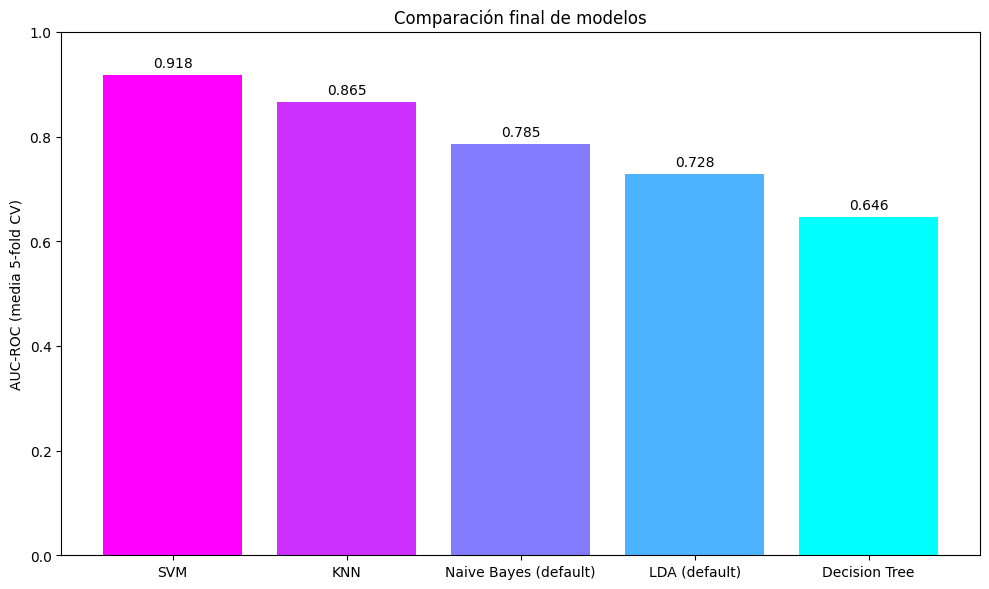
\includegraphics[width=0.60\linewidth]{img/comparacion-modelos.png}
    \caption*{Comparación final de mejores modelos}
    \label{fig:comparacion-modelos} 
\end{figure}


Observemos también que los modelos que consiguieron mejor performance fueron aquellos que se comportan mejor con una distribución normal de los datos, como es el caso de SVM utilizando el kernel radial, y modelos que asumen normalidad, como LDA y Naive Bayes. Además, KNN, que se basa en distancias, tuvo un rendimiento muy bueno, 
superior al de LDA y Naive Bayes, pero no tanto como el de SVM.